\section{谱的性质}
\label{sec:adjacency-spectral-properties}

上一节通过直接构造特征向量求出了几类典型图的完整谱。现在回到一般的图，研究邻接谱本身具有哪些普遍的结构性质。我们依次回答四个核心问题：
\begin{enumerate}
\item 最大特征值$\lambda_1$为什么地位特殊？它的重数是多少，对应的特征向量有什么符号特征？
\item 不必解出全部特征值，能否直接用顶点的度给出$\lambda_1$的上下界？
\item 从图中删去边、减小边权或删去顶点后，$\lambda_1$会如何变化？
\item 什么时候正特征值$\lambda$与负特征值$-\lambda$必定成对出现？
\end{enumerate}

本节在非负加权图的一般框架下统一讨论这些问题：设$\bm W=(w_{i,j})\in\mathbb R^{n\times n}$为非负实对称加权邻接矩阵（对角元$w_{i,i}=0$，边权$w_{i,j}=w_{j,i}\geq 0$）；简单无权图的邻接矩阵$\bm A$正是每条边权取$1$的特例。顶点$i$的加权度定义为第$i$行的边权之和$d_i=\sum_{j=1}^n w_{i,j}$。

\subsection{连通图的Perron定理}
\label{sec:adjacency-perron-theorem}

对实对称矩阵$\bm W$，其最大特征值$\lambda_1$可以通过单位球面上的Rayleigh商极值（可参考\BookChapterRef{chap:matrix-approximation}{卷二"矩阵逼近"章}）刻画为
\[
\lambda_1=\max_{\|\bm x\|_2=1}\bm x^\top\bm W\bm x.
\]
为了看清怎样的单位向量$\bm x=(x_1,\ldots,x_n)^\top$能让二次型$\bm x^\top\bm W\bm x$尽可能大，我们把矩阵二次型按图的边展开：
\[
\bm x^\top\bm W\bm x
=\sum_{i=1}^n\sum_{j=1}^n w_{i,j}x_i x_j
=2\sum_{\{i,j\}\in E}w_{i,j}x_i x_j.
\]
这里每一条无向边$\{i,j\}\in E$在双重大和中作为有序对$(i,j)$和$(j,i)$各出现一次，合并贡献$2w_{i,j}x_i x_j$。

观察单条正权边$\{i,j\}$（$w_{i,j}>0$）上的乘积项$2w_{i,j}x_i x_j$：如果两端顶点的赋值$x_i$与$x_j$正负号相反（例如一端取$+1$、另一端取$-1$），乘积$x_i x_j<0$，这条边就会给二次型带来负贡献$-2w_{i,j}|x_i||x_j|$，把总和往小里拉；反之，如果我们把向量$\bm x$的每一个分量都取绝对值，构造非负向量
\[
|\bm x|=\bigl(|x_1|,|x_2|,\ldots,|x_n|\bigr)^\top,
\]
那么一方面向量的欧氏长度完全不变：
\[
\bigl\||\bm x|\bigr\|_2=\sqrt{\sum_{i=1}^n |x_i|^2}=\sqrt{\sum_{i=1}^n x_i^2}=\|\bm x\|_2;
\]
另一方面，由于边权$w_{i,j}\geq 0$，每条边上的乘积都满足$w_{i,j}|x_i||x_j|\geq w_{i,j}x_i x_j$，因此二次型总和只会增大或保持不变：
\[
|\bm x|^\top\bm W|\bm x|
=2\sum_{\{i,j\}\in E}w_{i,j}|x_i||x_j|
\geq 2\sum_{\{i,j\}\in E}w_{i,j}x_i x_j
=\bm x^\top\bm W\bm x.
\]
这意味着：在单位球面上寻找最大化二次型的特征方向时，总可以选到各分量全非负的向量。

图~\ref{fig:adjacency-perron-absolute-value}在三点路径$1\!-\!2\!-\!3$（含两条单位权边$\{1,2\}$和$\{2,3\}$）上直观对比了取绝对值前后的效果。在图~\ref{fig:adjacency-perron-absolute-value}(a)中，取正负交替赋值$\bm x=(1,-1,1)^\top$，两条边的端点乘积均为$x_1x_2=x_2x_3=-1$，二次型为$\bm x^\top\bm A\bm x=2(-1)+2(-1)=-4$，Rayleigh商为$-4/3$；在图~\ref{fig:adjacency-perron-absolute-value}(b)中，逐分量取绝对值得到$|\bm x|=(1,1,1)^\top$，向量长度仍为$\sqrt{3}$，但两条边的端点乘积均变为$+1$，二次型跃升为$|\bm x|^\top\bm A|\bm x|=2(+1)+2(+1)=+4$，Rayleigh商提高到$+4/3$。

\begin{BookInlineFigure}
  \centering
  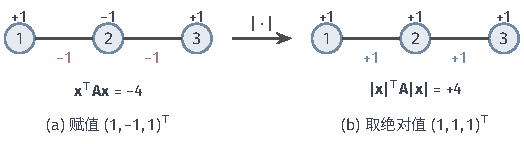
\includegraphics{figures/03-graphs/05-matrices-and-spectra/tikz/adjacency-perron-absolute-value/figure.pdf}
  \caption{三点路径$1\!-\!2\!-\!3$上逐分量取绝对值前后的二次型变化。边下方标注的是端点乘积$x_i x_j$。(a) 赋值$\bm x=(1,-1,1)^\top$时，两条边两端均异号，端点乘积为$-1$，二次型$\bm x^\top\bm A\bm x=2(-1-1)=-4$。(b) 取绝对值得到$|\bm x|=(1,1,1)^\top$后，向量长度不变，每条边的端点乘积变为$+1$，二次型升至$+4$。}
  \label{fig:adjacency-perron-absolute-value}
\end{BookInlineFigure}

在进入正式定理之前，我们先明确加权矩阵$\bm W$的连通条件。在矩阵乘向量$(\bm W\bm x)_i=\sum_{j=1}^n w_{i,j}x_j$中，若两个顶点$i,j$之间的权重$w_{i,j}=0$，则$x_j$对第$i$个输出分量没有任何贡献，二者在矩阵作用中互不相连；只有满足$w_{i,j}>0$的正权边才真正传递数值。为此给出正权支撑的正式定义。

\begin{definition}[正权支撑]
\label{def:positive-weight-support}
设$\bm W=(w_{i,j})\in\mathbb R^{n\times n}$为顶点集$V$上的非负对称邻接权矩阵（对角元$w_{i,i}=0$，边权$w_{i,j}=w_{j,i}\geq 0$）。保留全体顶点$V$、仅保留严格正权边
\begin{equation}
E_+=\bigl\{\{i,j\}\subseteq V:w_{i,j}>0\bigr\}
\label{eq:positive-weight-support}
\end{equation}
所构成的无权简单图$\mathcal G_+=(V,E_+)$称为加权图（或矩阵$\bm W$）的\term{正权支撑}（positive-weight support）。
\end{definition}

当正权支撑$\mathcal G_+$连通时，任意两个顶点之间都存在一条每步边权均严格大于零的路径，非零读数才能沿正权路径传遍全图所有顶点。

\begin{theorem}[连通图的Perron定理]
\label{thm:adjacency-perron}
设$\bm W=(w_{i,j})\in\mathbb R^{n\times n}$为有限无向图的非负对称邻接权矩阵，且其正权支撑$\mathcal G_+$连通（$n\geq 2$）。则：
\begin{enumerate}
\item 最大特征值$\lambda_1>0$的代数重数为$1$，且存在各分量均严格为正的特征向量$\bm p=(p_1,\ldots,p_n)^\top$（$p_i>0,\forall i$）；
\item $\bm W$的任意特征值$\lambda$均满足$|\lambda|\leq\lambda_1$（即谱半径等于$\lambda_1$）。
\end{enumerate}
\end{theorem}

\begin{proof}
我们分三步依次证明：（1）存在各分量严格为正的最大特征向量$\bm p$；（2）最大特征值$\lambda_1$的特征空间是一维的（重数为$1$）；（3）其余特征值均满足$|\lambda|\leq\lambda_1$。

\textbf{第一步（严格正特征向量的存在性）}：在单位球面$\|\bm x\|_2=1$上任取一个使Rayleigh商达到最大值$\lambda_1$的单位特征向量$\bm x$，令$\bm p=|\bm x|$。由前面的绝对值不等式，有
\[
\lambda_1\geq\bm p^\top\bm W\bm p
=\sum_{i,j}w_{i,j}|x_i||x_j|
\geq\sum_{i,j}w_{i,j}x_i x_j
=\bm x^\top\bm W\bm x=\lambda_1,
\]
且$\|\bm p\|_2=\|\bm x\|_2=1$。因此$\bm p^\top\bm W\bm p=\lambda_1$，即非负单位向量$\bm p$也在单位球面上达到最大Rayleigh商$\lambda_1$。由Rayleigh商在极值点处的驻点条件，$\bm p$本身就是属于最大特征值$\lambda_1$的特征向量：$\bm W\bm p=\lambda_1\bm p$。又因正权支撑连通且$n\geq 2$，图中至少有一条正权边，取常向量即可见$\lambda_1>0$。

下面用反证法说明$\bm p$不可能含有零分量。假设存在某个顶点$i$使得$p_i=0$。读取特征方程$\bm W\bm p=\lambda_1\bm p$的第$i$行：
\[
0=\lambda_1 p_i=\sum_{j=1}^n w_{i,j}p_j.
\]
由于右端每一项都满足$w_{i,j}\geq 0$且$p_j\geq 0$，非负项之和等于零迫使每一项都等于零。特别地，对顶点$i$在正权支撑中的每一个邻居$j$（满足$w_{i,j}>0$），都必有$p_j=0$。也就是说，“分量为零”这一性质会从顶点$i$传播到它的所有正权邻居。由于正权支撑$\mathcal G_+$连通，从$i$出发沿正权路径逐歩传递，最终推出全图所有顶点的分量都满足$p_k=0$（$\forall k\in V$），即$\bm p=\bm 0$，这与$\|\bm p\|_2=1$矛盾。因此$\bm p$的每个分量都严格为正：$p_i>0$（$\forall i\in V$）。

\textbf{第二步（$\lambda_1$的重数为$1$）}：用反证法。假设$\lambda_1$的特征子空间维数大于$1$，则可以在该特征子空间中选出一个与$\bm p$正交的单位特征向量$\bm y$（满足$\bm W\bm y=\lambda_1\bm y$，$\|\bm y\|_2=1$，且$\langle\bm p,\bm y\rangle=0$）。

对$\bm y$重复第一步的推导：令$|\bm y|=(|y_1|,\ldots,|y_n|)^\top$，则$|\bm y|$也是属于$\lambda_1$的非负单位特征向量；再由第一步的零分量传播论证，可知$|\bm y|$的每个分量都严格为正，从而$\bm y$的每个分量都非零（$y_i\neq 0,\forall i\in V$）。

另一方面，由于$|\bm y|^\top\bm W|\bm y|=\bm y^\top\bm W\bm y=\lambda_1$，不等式
\[
\sum_{\{i,j\}\in E}2w_{i,j}|y_i||y_j|
\geq\sum_{\{i,j\}\in E}2w_{i,j}y_i y_j
\]
必须取等号。因为每一条边上的差$2w_{i,j}(|y_i||y_j|-y_i y_j)\geq 0$都非负，总和为零要求每一条正权边$\{i,j\}\in E_+$（$w_{i,j}>0$）都满足$|y_i||y_j|=y_i y_j$。由于$y_i\neq 0$且$y_j\neq 0$，这意味着正权边的两个端点$y_i$与$y_j$必须严格同号。沿连通的正权支撑传递，向量$\bm y$的所有$n$个分量必定同为正数或同为负数。然而$\bm p$的所有分量严格为正，于是内积$\langle\bm p,\bm y\rangle=\sum_{i=1}^n p_i y_i$是$n$个严格同号非零项之和，绝不可能等于$0$——这与$\langle\bm p,\bm y\rangle=0$矛盾。故$\lambda_1$的特征空间只能是一维的，重数为$1$。

\textbf{第三步（谱半径界$|\lambda|\leq\lambda_1$）}：任取$\bm W$的一个特征值$\lambda$及其单位特征向量$\bm z$（$\|\bm z\|_2=1$）。由三角不等式与$\lambda_1$的极大性质，
\[
|\lambda|
=|\bm z^\top\bm W\bm z|
=\Bigl|\sum_{i,j}w_{i,j}z_i z_j\Bigr|
\leq\sum_{i,j}w_{i,j}|z_i||z_j|
=|\bm z|^\top\bm W|\bm z|
\leq\lambda_1,
\]
定理证毕。
\end{proof}

定理~\ref{thm:adjacency-perron}中唯一确定的严格正单位特征向量$\bm p$称为图的\term{Perron向量}（Perron vector）。需要注意，定理保证最大特征值$\lambda_1$本身是单根，但并不排除最小特征值$\lambda_n$达到相反数$-\lambda_1$（此时$|\lambda_n|=\lambda_1$）。例如单边图$K_2$的特征值为$+1$和$-1$。第~\ref{sec:adjacency-bipartite-symmetry}小节将证明：在正权支撑连通图上，$\lambda_n=-\lambda_1$发生当且仅当该图是二部图。

\subsection{谱的上下界}
\label{sec:adjacency-degree-bounds}

Perron定理确立了最大特征值$\lambda_1$的单根性与正特征向量，但在一般非正则图上并不能直接写出$\lambda_1$的闭式解。下面我们分别利用Rayleigh商的下界性质和Perron向量的最大分量，证明$\lambda_1$始终被夹在图的平均度$\overline d$与最大度$d_{\max}$之间。

\paragraph{下界：用全一常向量测试Rayleigh商}

根据Rayleigh商的极大性质，最大特征值$\lambda_1$是$\frac{\bm x^\top\bm W\bm x}{\bm x^\top\bm x}$在所有非零向量$\bm x\neq\bm 0$上的最大值：
\[
\lambda_1=\max_{\bm x\neq\bm 0}\frac{\bm x^\top\bm W\bm x}{\bm x^\top\bm x}.
\]
因此，我们随便挑选一个具体的非零向量$\bm x$代进去算出的Rayleigh商，都必然小于或等于最大值$\lambda_1$。

取最简单的全一常向量$\bm x=\bm 1=(1,1,\ldots,1)^\top\in\mathbb R^n$（所有顶点赋相同的读数$1$），分两步计算它的Rayleigh商。先算矩阵乘向量$\bm W\bm 1$：按矩阵乘法规则，$\bm W\bm 1$的第$i$个分量是把$\bm W$第$i$行的所有元素各自乘以$1$再相加：
\[
(\bm W\bm 1)_i=\sum_{j=1}^n w_{i,j}\cdot 1=\sum_{j=1}^n w_{i,j}=d_i.
\]
也就是说，对全一向量$\bm 1$作用一次邻接矩阵$\bm W$，输出向量的第$i$个分量恰好就是顶点$i$的加权度$d_i$，即$\bm W\bm 1=(d_1,d_2,\ldots,d_n)^\top$（若改用单位化常向量$\bm u=\frac{1}{\sqrt n}\bm 1$，则输出的第$i$个分量为$d_i/\sqrt n$）。

再算二次型与Rayleigh商：用行向量$\bm 1^\top$左乘输出向量$\bm W\bm 1$，相当于把全部$n$个顶点的度相加：
\[
\bm 1^\top\bm W\bm 1=\sum_{i=1}^n 1\cdot(\bm W\bm 1)_i=\sum_{i=1}^n d_i.
\]
而全一向量本身的长度平方为$\bm 1^\top\bm 1=\sum_{i=1}^n 1^2=n$。将两者相除，就得到全一向量$\bm 1$的Rayleigh商恰好等于全图的平均度$\overline d$：
\[
\frac{\bm 1^\top\bm W\bm 1}{\bm 1^\top\bm 1}
=\frac{1}{n}\sum_{i=1}^n d_i
=\overline d.
\]
在简单无权图中，每条无向边为两个端点的度各贡献$1$，总度数$\sum_{i=1}^n d_i=2m$，故平均度为$\overline d=2m/n$。由于最大值$\lambda_1$不小于特定向量$\bm 1$的Rayleigh商，立即得到下界：
\[
\lambda_1\geq\overline d.
\]

\paragraph{上界：在Perron向量的最大分量处放缩}

再证上界$\lambda_1\leq d_{\max}$，其中$d_{\max}=\max_{1\leq i\leq n}d_i$为全图的最大度。取属于$\lambda_1$的非负特征向量$\bm p=(p_1,\ldots,p_n)^\top\neq\bm 0$（连通图上即为严格正的Perron向量），并在全部$n$个顶点中找出分量最大的那个顶点$i^\star$，使得
\[
p_{i^\star}=\max_{1\leq j\leq n}p_j>0.
\]
写出特征方程$\bm W\bm p=\lambda_1\bm p$在顶点$i^\star$这一行的等式，并将右端每个邻居的分量$p_j$放大为最大值$p_{i^\star}$（注意到$w_{i^\star,j}\geq 0$）：
\[
\lambda_1 p_{i^\star}
=\sum_{j=1}^n w_{i^\star,j}\,p_j
\leq\sum_{j=1}^n w_{i^\star,j}\,p_{i^\star}
=\Bigl(\sum_{j=1}^n w_{i^\star,j}\Bigr)p_{i^\star}
=d_{i^\star}\,p_{i^\star}
\leq d_{\max}\,p_{i^\star}.
\]
因为$p_{i^\star}>0$，在不等式两端同除以正数$p_{i^\star}$，即得上界$\lambda_1\leq d_{\max}$。

\begin{theorem}[最大邻接特征值的度界]
\label{prop:adjacency-degree-bounds}
对任意非负实对称邻接矩阵$\bm W\in\mathbb R^{n\times n}$，其最大特征值$\lambda_1$满足
\begin{equation}
\overline d\leq\lambda_1\leq d_{\max}.
\label{eq:adjacency-degree-spectral-bounds}
\end{equation}
若$\bm W$的正权支撑连通，则$\lambda_1=\overline d$（或$\lambda_1=d_{\max}$）成立当且仅当图中所有顶点的加权度均相等（即图为正则图）。
\end{theorem}

\paragraph{取等条件}

我们来追踪正权支撑连通时式~\eqref{eq:adjacency-degree-spectral-bounds}两端何时取等号。若上界$\lambda_1=d_{\max}$取等，则前面关于最大分量顶点$i^\star$的两步放缩必须同时取等号：第一步等号$\sum_j w_{i^\star,j}(p_{i^\star}-p_j)=0$要求$i^\star$的每一个正权邻居$j$（$w_{i^\star,j}>0$）都达到最大分量$p_j=p_{i^\star}$，第二步等号要求$d_{i^\star}=d_{\max}$。既然正权邻居$j$也达到了最大分量$p_j=p_{i^\star}$，对顶点$j$再次应用同样的推理，可知$d_j=d_{\max}$且$j$的所有正权邻居分量也等于$p_{i^\star}$。沿连通的正权支撑传遍全图，所有顶点的度都必须等于$d_{\max}$，图必为正则图。

若下界$\lambda_1=\overline d$取等，则说明常向量$\bm 1$的Rayleigh商已经达到了全局最大值$\lambda_1$，因此$\bm 1$本身就是属于$\lambda_1$的特征向量，满足$\bm W\bm 1=\overline d\,\bm 1$。逐分量读取该式，即得对所有顶点$i$都有$d_i=(\bm W\bm 1)_i=\overline d$，图同样是正则图。

以三点路径$P_3$和四点环$C_4$对照：$P_3$的度序列为$(1,2,1)$，平均度$\overline d=4/3\approx 1.333$，最大特征值$\lambda_1=\sqrt 2\approx 1.414$，最大度$d_{\max}=2$，满足严格不等式$4/3<\sqrt 2<2$；而$2$正则图$C_4$的度序列为$(2,2,2,2)$，三者相等$\overline d=\lambda_1=d_{\max}=2$。

\subsection{子图的谱单调性}
\label{sec:adjacency-spectral-monotonicity}

如果在图中删去一条边、降低某条边的正权重，或者删去一个顶点及其关联边，每个顶点的邻居贡献只减不增。下面用非负最大化向量证明：最大特征值$\lambda_1$对子图具有单调性，且在连通图上删去任何正权边或顶点都会使$\lambda_1$严格下降。

设$\bm W'\in\mathbb R^{n\times n}$是由$\bm W\in\mathbb R^{n\times n}$减小部分边权（包括将边权降为$0$以表示删边，或将某个被删顶点的整行整列置为$0$）所得的非负对称矩阵，满足逐元素$0\leq w'_{i,j}\leq w_{i,j}$。在$\bm W'$上取一个非负单位特征向量$\bm x\geq\bm 0$（$\|\bm x\|_2=1$）使得$\bm x^\top\bm W'\bm x=\lambda_1(\bm W')$。将同一个非负单位向量$\bm x$代入原矩阵$\bm W$的二次型比较：
\[
\lambda_1(\bm W')
=\bm x^\top\bm W'\bm x
=\sum_{i,j}w'_{i,j}x_i x_j
\leq\sum_{i,j}w_{i,j}x_i x_j
=\bm x^\top\bm W\bm x
\leq\lambda_1(\bm W).
\]
这里第一个不等式来自$0\leq w'_{i,j}\leq w_{i,j}$与$x_i x_j\geq 0$，第二个不等式来自$\lambda_1(\bm W)$是$\bm W$在单位球面上的最大Rayleigh商。

进一步，若原图$\bm W$的正权支撑连通，且$\bm W'\neq\bm W$（确实减小了至少一条边$\{u,v\}$的权重$w'_{u,v}<w_{u,v}$），能否出现等号$\lambda_1(\bm W')=\lambda_1(\bm W)$？若两端相等，则上面不等式链中的两处不等号都必须取等：一方面，第二处取等$\bm x^\top\bm W\bm x=\lambda_1(\bm W)$说明$\bm x$也是连通矩阵$\bm W$达到$\lambda_1(\bm W)$的单位特征向量，由定理~\ref{thm:adjacency-perron}（Perron定理）知$\bm x$的每一个分量都严格为正（$x_i>0,\forall i\in V$）；另一方面，既然$x_u>0$且$x_v>0$，在权重严格减小的那条边$\{u,v\}$上就有$w'_{u,v}x_u x_v<w_{u,v}x_u x_v$，导致第一处不等式严格成立$\bm x^\top\bm W'\bm x<\bm x^\top\bm W\bm x$，产生矛盾。因此，在正权支撑连通图上，删去任意正权边、降低任意正权边的权重，或删去任意顶点，都会使最大邻接特征值严格减小：$\lambda_1(\bm W')<\lambda_1(\bm W)$。

例如从$n$点环$C_n$中删去一条边得到路径$P_n$，最大特征值从$\lambda_1(C_n)=2$严格下降为$\lambda_1(P_n)=2\cos\bigl(\frac{\pi}{n+1}\bigr)<2$。反之，若原图不连通，例如取$\mathcal G=C_4\sqcup K_2$，其最大特征值$\lambda_1=2$由$C_4$分量单独决定；此时删去较小分量$K_2$中的边并不会改变全图的最大特征值$\lambda_1=2$，这说明严格单调性确实依赖原图的连通性假设。

\subsection{二部图的谱对称性}
\label{sec:adjacency-bipartite-symmetry}

前面三小节聚焦于谱右端的最大特征值$\lambda_1$。现在我们把目光转向整个邻接谱的左右两端：在什么条件下，图的邻接谱关于原点对称（即每个特征值$\lambda$与$-\lambda$以相同重数成对出现）？答案恰好刻画了二部图。

先看二部图为什么必然具有对称谱。设图$\mathcal G$是二部图，其顶点集划分为左右两个独立集$V=X\cup Y$，所有正权边都横跨在$X$与$Y$之间（同侧内部没有任何正权边）。我们构造一个$n\times n$对角符号矩阵$\bm S=\operatorname{diag}(s_1,\ldots,s_n)$：
\[
s_i=
\begin{cases}
+1,& i\in X,\\
-1,& i\in Y.
\end{cases}
\]
显然$\bm S^\top=\bm S$且$\bm S^2=\bm I$（$\bm S$是正交对合矩阵）。考察正交相似变换$\bm S\bm W\bm S$的第$(i,j)$个元素$s_i w_{i,j}s_j$：当$w_{i,j}>0$时，边$\{i,j\}$连接$X$与$Y$异侧端点，必有$s_i s_j=(+1)(-1)=-1$，故$s_i w_{i,j}s_j=-w_{i,j}$；当$w_{i,j}=0$时，同样有$s_i w_{i,j}s_j=0=-w_{i,j}$。因此，对角符号矩阵$\bm S$把整个邻接权矩阵$\bm W$变成了它的相反数：
\begin{equation}
\bm S\bm W\bm S=-\bm W,\qquad\text{或等价地}\qquad \bm W\bm S=-\bm S\bm W.
\label{eq:adjacency-bipartite-anticommute}
\end{equation}

利用式~\eqref{eq:adjacency-bipartite-anticommute}，若$\bm x$是$\bm W$属于特征值$\lambda$的特征向量（$\bm W\bm x=\lambda\bm x$），将$\bm W$作用在翻转了$Y$侧符号的向量$\bm S\bm x$上：
\[
\bm W(\bm S\bm x)=-\bm S\bm W\bm x=-\bm S(\lambda\bm x)=(-\lambda)(\bm S\bm x).
\]
这表明$\bm S\bm x$正是$\bm W$属于相反数特征值$-\lambda$的特征向量。图~\ref{fig:adjacency-bipartite-sign-flip}在四元环$C_4$（二部划分$X=\{1,3\},Y=\{2,4\}$）上展示了这一操作：将属于$\lambda=+2$的特征向量$\bm x=(1,1,1,1)^\top$在$Y$侧变号，立即得到属于$-\lambda=-2$的特征向量$\bm S\bm x=(1,-1,1,-1)^\top$。由于可逆矩阵$\bm S$在$\lambda$的特征子空间与$-\lambda$的特征子空间之间建立了线性同构，两个特征值$\lambda$与$-\lambda$的代数重数必然完全相等，即整个邻接谱关于原点对称：$\lambda_i=-\lambda_{n+1-i}$（$i=1,\ldots,n$）。

\begin{BookInlineFigure}
  \centering
  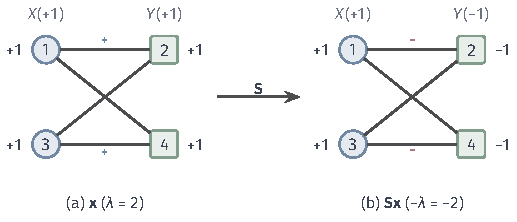
\includegraphics{figures/03-graphs/05-matrices-and-spectra/tikz/adjacency-bipartite-sign-flip/figure.pdf}
  \caption{二部图上的对角符号翻转$\bm S\bm W\bm S=-\bm W$（以$C_4$为例，圆点为$X=\{1,3\}$，方点为$Y=\{2,4\}$）。(a) 属于特征值$\lambda=+2$的特征向量$\bm x=(1,1,1,1)^\top$，跨部边两端同号。(b) 经$\bm S$保持$X$侧符号、翻转$Y$侧符号后，跨部边两端全部反号，得到属于特征值$-\lambda=-2$的特征向量$\bm S\bm x=(1,-1,1,-1)^\top$。}
  \label{fig:adjacency-bipartite-sign-flip}
\end{BookInlineFigure}

反过来，谱关于原点对称（甚至在连通图上仅最小特征值满足$\lambda_n=-\lambda_1$）也能反推出图是二部图。

\begin{theorem}[二部图的谱对称性]
\label{thm:adjacency-bipartite-spectral-symmetry}
设$\bm W\in\mathbb R^{n\times n}$为有限无向无自环图的非负对称邻接权矩阵。则以下命题成立：
\begin{enumerate}
\item $\bm W$的邻接谱关于零对称（即对每个$i=1,\ldots,n$都有$\lambda_i=-\lambda_{n+1-i}$），当且仅当其正权支撑$\mathcal G_+$是二部图（不含奇数长度的环）；
\item 若进一步$\bm W$的正权支撑连通且$n\geq 2$，则只需两端特征值满足$\lambda_n=-\lambda_1$，即可判定正权支撑$\mathcal G_+$是二部图。
\end{enumerate}
\end{theorem}

\begin{proof}
\textbf{第1条}：充分性（二部图$\implies$谱关于零对称）已由式~\eqref{eq:adjacency-bipartite-anticommute}给出。下面证明必要性（谱关于零对称$\implies$不含奇环）：若邻接谱关于零对称，则对任意正奇数$k=1,3,5,\ldots$，每一对相反特征值$\lambda$与$-\lambda$的奇数次幂滿足$(-\lambda)^k=-\lambda^k$，相加相互抵消（零特征值的幂本身为$0$），因此所有奇数阶谱矩恒等于零：
\[
\operatorname{tr}(\bm W^k)=\sum_{i=1}^n\lambda_i^k=0,\qquad k=1,3,5,\ldots.
\]
假设正权支撑$\mathcal G_+$中含有一个奇数长度$\ell$的简单环$v_1\to v_2\to\cdots\to v_\ell\to v_1$。沿该奇环绕行一圈是一条长度为$\ell$的闭行走，其沿途每一步的边权均严格为正，乘积$w_{v_1,v_2}w_{v_2,v_3}\cdots w_{v_\ell,v_1}>0$为$(\bm W^\ell)_{v_1,v_1}$贡献了一个严格正数。由于$\bm W$的所有元素非负，其余一切$\ell$步闭行走的权重乘积均非负，不可能抵消这一正贡献，从而$\operatorname{tr}(\bm W^\ell)>0$，与奇数阶迹为零矛盾。故正权支撑$\mathcal G_+$中不含奇环，必为二部图。

\textbf{第2条}：设正权支撑$\mathcal G_+$连通（$n\geq 2$，从而$\lambda_1>0$）且$\lambda_n=-\lambda_1$。取属于最小特征值$\lambda_n$的实单位特征向量$\bm x$（$\bm W\bm x=\lambda_n\bm x$，$\|\bm x\|_2=1$），则$\bm x^\top\bm W\bm x=\lambda_n=-\lambda_1$。考察绝对值向量$|\bm x|=(|x_1|,\ldots,|x_n|)^\top$的二次型：
\[
\begin{aligned}
\lambda_1
&\geq|\bm x|^\top\bm W|\bm x|
=\sum_{i,j}w_{i,j}|x_i||x_j|
\geq\Bigl|\sum_{i,j}w_{i,j}x_i x_j\Bigr|\\
&=|\bm x^\top\bm W\bm x|
=-\bm x^\top\bm W\bm x
=-\lambda_n=\lambda_1.
\end{aligned}
\]
首尾两端相等迫使中间不等式全部取等号。首先，$|\bm x|^\top\bm W|\bm x|=\lambda_1$说明非负单位向量$|\bm x|$达到了最大特征值$\lambda_1$；由定理~\ref{thm:adjacency-perron}（Perron定理），$|\bm x|$是严格正的Perron向量，故$|x_i|>0$（即$x_i\neq 0,\forall i\in V$）。其次，$\sum_{i,j}w_{i,j}|x_i||x_j|=\sum_{i,j}w_{i,j}(-x_i x_j)$等价于
\[
\sum_{\{i,j\}\in E_+}2w_{i,j}\bigl(|x_i||x_j|+x_i x_j\bigr)=0.
\]
由于对每条边都有$|x_i||x_j|+x_i x_j\geq 0$且正权边满足$w_{i,j}>0$，每一条正权边$\{i,j\}\in E_+$都必须满足
\[
x_i x_j=-|x_i||x_j|<0.
\]
这意味着：每条正权边的两个端点在向量$\bm x$中的分量符号必定一正一负。令
\[
X=\{i\in V:x_i>0\},\qquad Y=\{i\in V:x_i<0\},
\]
由于每个$x_i\neq 0$，$V=X\cup Y$构成顶点集的一个划分，且所有正权边都连接$X$中的顶点与$Y$中的顶点，$X$与$Y$内部均无正权边。因此正权支撑$\mathcal G_+$是二部图。
\end{proof}

对比两个例子：四元环$C_4$的谱为$\{2,0,0,-2\}$，关于零对称且$\lambda_4=-2=-\lambda_1$，是二部图；三角形$C_3$的谱为$\{2,-1,-1\}$，不关于零对称且$\lambda_3=-1\neq -\lambda_1$，含有奇环。同时要注意第2条中“正权支撑连通”这一前提不可省略：若取不连通图$\mathcal G=C_3\sqcup K_{3,3}$，其中$C_3$的谱为$\{2,-1,-1\}$、二部图分量$K_{3,3}$的谱为$\{3,0,0,0,0,-3\}$，合在一起全图最大特征值$\lambda_1=3$与最小特征值$\lambda_9=-3$依然满足$\lambda_9=-\lambda_1$，但整张图因包含三角形分量$C_3$而不是二部图（此时完整谱中由$C_3$贡献的$+2$没有对应的$-2$，按第1条的完整谱对称性仍能准确排除二部性）。
